% !TeX root = ../main.tex
\chapter{绪论}
\section{研究背景及意义}
无人飞行器(Unmanned Aerial Vehicle, UAV),是利用无线电遥控设备和自备的程序控制装置操纵的不载人飞行器。无人飞行器可以通过携带各种各样的设备来执行不同的任务,与载人飞机相比,它具有以下优点:\par
\begin{enumerate}
	\item 设计成本低。无人飞行器由于无需驾驶员,所有减少了驾驶舱及其相应设计设备的成本开发,取而代之的是一个飞行控制器,两者相比较而言,大大减少了成本费用。
	\item 载重能力强。由于减少了驾驶员及驾驶舱及其设备,无人飞行器的载重能力因此增强,而且可以不再考虑驾驶员的生理极线,相比较而言,机动能力大大提高,能完成以前不能完成的动作。
	\item 应用范围广,使用方便。无人飞行器能根据各种各样的机载设备来完成不同的任务,并且对环境的要求较低,因此可以在复杂环境下完成各种任务。
	由于无人飞行器的以上优点,使得无人飞行器受到各国各界的关注并开展了一系列的研发工作,大大加快了无人飞行器的发展。
\end{enumerate}\par
近年来,无人飞行器在军用和民用领域中的应用越来越广泛,例如在民用邻域中的环境检测、电力巡检;在军用领域中的边境巡逻、灾情检测等任务。在这些任务中,能否有效获取无人飞行器的位置信息以及周围环境信息很大程度上决定了任务能否有效完成预定任务。因此,无人飞行器的定位与周围环境感知技术成为了无人飞行器研究邻域的重要研究领域之一。传统的解决方案是利用GPS加上IMU的惯性导航系统来获取无人飞行器的位姿、速度等相关信息。但这样存在一定的局限性,例如GPS在室内环境和城市高楼、山地峡谷间等环境下会因信号弱而导致无法工作,而IMU则会跟随时间的推移引起较大的累计误差造成无人飞行器定位不准确。
\begin{figure}[htbp]
	\centering
	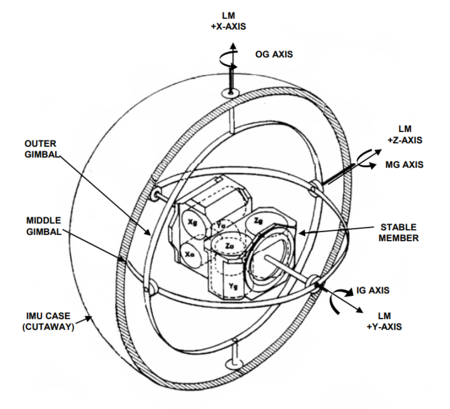
\includegraphics[height=5cm]{imu}
	\caption{IMU惯导平台的结构}
\end{figure}\par
在无人飞行器的定位与环境感知领域中,视觉传感器是一种能为定位与环境感知提供大量信息的传感器。随着制作工艺的发展,视觉传感器也越来越小,重量也越来越轻,性能则越来越强,因此也逐渐成为这个领域的研究热点。它最初是在机器人领域中被提出,但是由于无人飞行器的快速发展,逐渐也运用在这个领域中。视觉定位与环境感知主要由摄像头采集环境图像,将图像传送给图像处理器,获取无人飞行器的相对位姿,利用相关地图绘制算法生成相应的地图,从而获取周围环境信息,为接下来的任务提供信息支持。\par
同步定位与建图(Simultaneous Localization and Mapping,SLAM)算法,利用移动平台的机载摄像机在未知环境中建立一个地图,并由此地图计算出移动平台的位姿及运动轨迹。本文的目标就是研究视觉传感器的SLAM算法,利用视觉传感器完成对无人飞行器的定位以及周围环境地图的构建。
\section{视觉SLAM系统概述}
SLAM自1986年诞生以来,一直以来是人工智能领域的热点问题。关于它的文献数以千计,SLAM也涉及到很多数学和计算机科学等多学科的知识,例如微分几何、射影几何、机器视觉、随机过程、位姿状态估计理论、李群李代数等,将这些知识精妙的糅合在一起,通过程序去实现相关的理论算法。由于其重要的理论与应用价值,被很多学者认为是实现真正全自主移动机器人的关键。
\par
\section{SLAM系统的标准模型}
\begin{figure}[htbp]
	\centering
	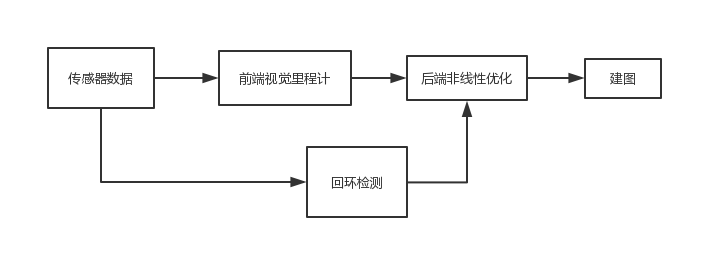
\includegraphics[height=5cm]{pipline}
	\caption{经典SLAM流程}
	\label{fig:pipline}
\end{figure}\par
经典的视觉SLAM框架如图\ref{fig:pipline}所示:\par
\begin{enumerate}
	\item 传感器数据。主要为视觉传感器的图像数据或者其他例如惯性传感器的数据以及图像信息的读取和预处理。
	\item 前端视觉里程计。估计相邻时刻相机运动以及构建局部地图。
	\item 后端非线性优化。后端接受不同时刻前端测量的相机位姿、环境信息以及回环检测的信息,对它们进行优化,得到全局一致的轨迹和地图。
	\item 回环检测。回环检测判断机器人是否曾经路过一样的地方。如果检测到曾经过相似场景,将信息提供给后端进行非线性优化。
	\item 建图。根据估计的机器人位姿和运动轨迹,建立所需的地图。
\end{enumerate}
总而言之,视觉SLAM的工作就是获取相机图像,对图像进行处理,然后经过一系列的算法获得相机的位姿和运动轨迹,然后根据获得的相机位姿和运动轨迹建立我们需要的地图。\par
一般而言,视觉传感器就是摄像机,而我们从摄像机获得的数据是有畸变的。所以我们首先要对摄像机进行标定,获得相机标定参数,用这些参数处理图像,这样我们才能获得我们所需要的无畸变的图像。\par
在获得我们所需要的图像信息后,我们就要建立视觉里程计。视觉里程计的主要作用就是估计相邻图像的相机运动,具体而言就是相机转了多少度,平移了多少。对于计算机来说,这些东西就是一个个矩阵,我们所需要做的就是根据相机和几何点的关系获取这些矩阵。\par
前端视觉里程计能够根据相邻时刻的图像估计相邻图像的位姿和运动轨迹,并解析出三维空间场景。那么很自然的我们就能想到我们可以根据相邻图像的位姿和运动轨迹还原整个运动过程的位姿变换、运动轨迹以及观测到的路标点的空间位置。我们将获得的这些信息保存下来,如图\ref{fig:benchmark}所示。这样我们就获得了一张由相机估计出来的地图,完成了建图任务。
\begin{figure}[H]
	\centering
	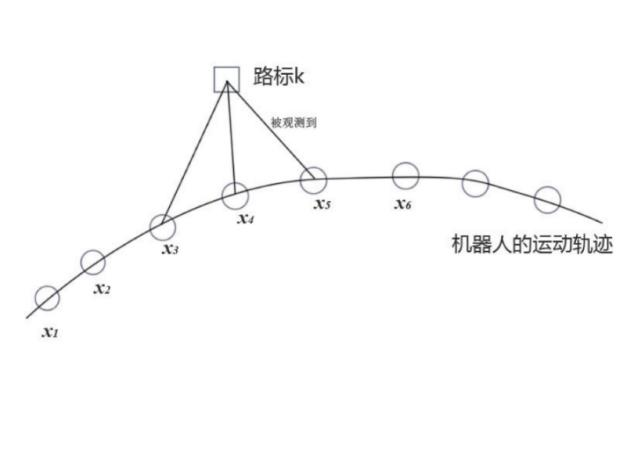
\includegraphics[height=8cm]{benchmark}
	\caption{机器人轨迹}
	\label{fig:benchmark}
\end{figure}\par
然而仅通过视觉里程计建立的地图将不可避免的出现累计误差。这个原因是视觉里程计只通过相邻的图像来估计相机位姿和运动轨迹,但是我们知道每次估计都毫无疑问的会有误差,而由于视觉里程计的工作方式,这些先前时刻产生的误差又会传递到下一时刻。这样经过一段时间之后,估计的轨迹边不再准确,如图\ref{fig:error}所示。
\begin{figure}[H]
	\centering
	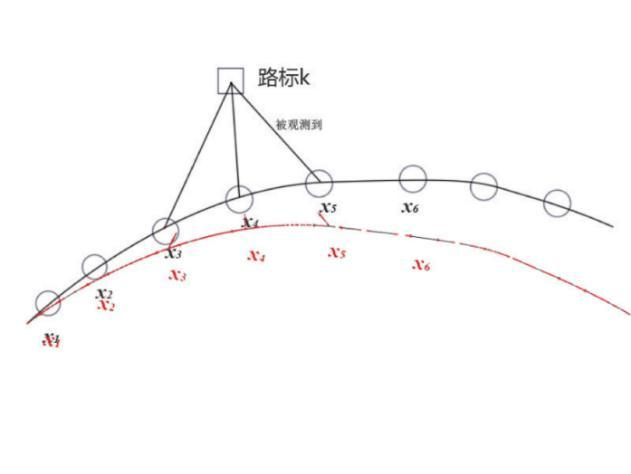
\includegraphics[height=8cm]{error}
	\caption{机器人实际轨迹和估计轨迹}
	\label{fig:error}
\end{figure}\par
这就是所谓的漂移,导致我们无法建立一致的地图。最直观的表现就是,原本之的走廊变成了斜的,这实在是一个让人难以忍受的事情。所以为了解决这个漂移问题,我们还需要两种技术:后端优化和回环检测。如图\ref{fig:ldc}所示,左边是累计误差未处理估计的运动轨迹,右图是经过回环检测后估计的运动轨迹。
\begin{figure}[H]
	\centering
	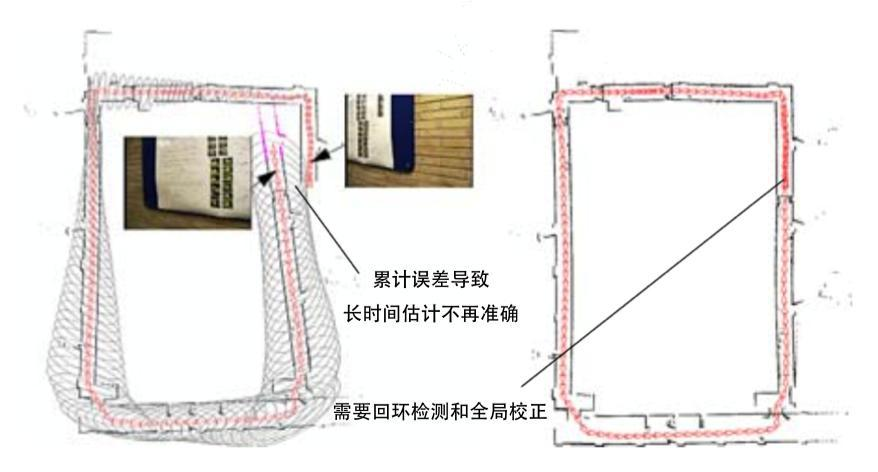
\includegraphics[height=8cm]{loopdetectioncorrection}
	\caption{回环检测示意图}
	\label{fig:ldc}
\end{figure}\par

后端优化,主要指的是处理SLAM过程中的噪声问题。虽然我们很希望所有的数据是准确的,但是在现实中,就算再准确地传感器都会有噪声,并且还容易受外界环境的影响,比如磁场、温度等。所有在一个完整的视觉SLAM框架中,我们不只要关注“如何从图像估计出相机运动”,还要关心这个估计带有多大的噪声,这些噪声是如何从上一时刻到传递到下一时刻,而我们对这个估计又有多大的自信。
\par
后端优化要考虑的问题就是如何从带有噪声的数据中估计整个系统的状态,以及这个状态的不确定性。后端负责的是整个SLAM的优化过程,往往面对的只有数据,而并不关心这些数据到底来自哪些传感器。
\par
回环检测(Loop Closure Detection),主要解决的是位置估计随着时间漂移的问题。具体办法是让系统在一段时间后来到它曾经到过的相似的场景,并与当前帧进行配对,再把之前错误的估计消除掉,这样就能得到比较准确的整个运动过程的位姿和轨迹还有构建的地图了。
\par
事实上,地图存在的意义不只是单纯的为了重建场景,还有就是为了让系统认路(识别曾今到过的场景),来实现回环检测。实现的手段很多,例如我们可以在无人飞行器下方设置一个标志物,只要看到这个标志物,就知道这个无人飞行器飞到了相对于这个标志物的方位。但这个标志物其实是一个环境传感器,对应用环境做了限制。我们更希望由系统携带的传感器来完成这一任务,例如可以利用图像间的相似性来完成回环检测。在检测到回环之后,我们会把这些信息告诉后端,然后后端根据这些新的信息把估计轨迹和地图调整到符合回环检测结果的样子。这样如果我们有充分而且正确的回环检测,就可以消除累计误差,得到全局一致的轨迹和地图。\par
建图(Mapping),是指SLAM地图的构建。这里的地图指的是对环境的描述,并不是固定的,而是视SLAM的应用而定。例如,图\ref{fig:maps}就是根据需要建立的各种各样的地图。
\begin{figure}[H]
	\centering
	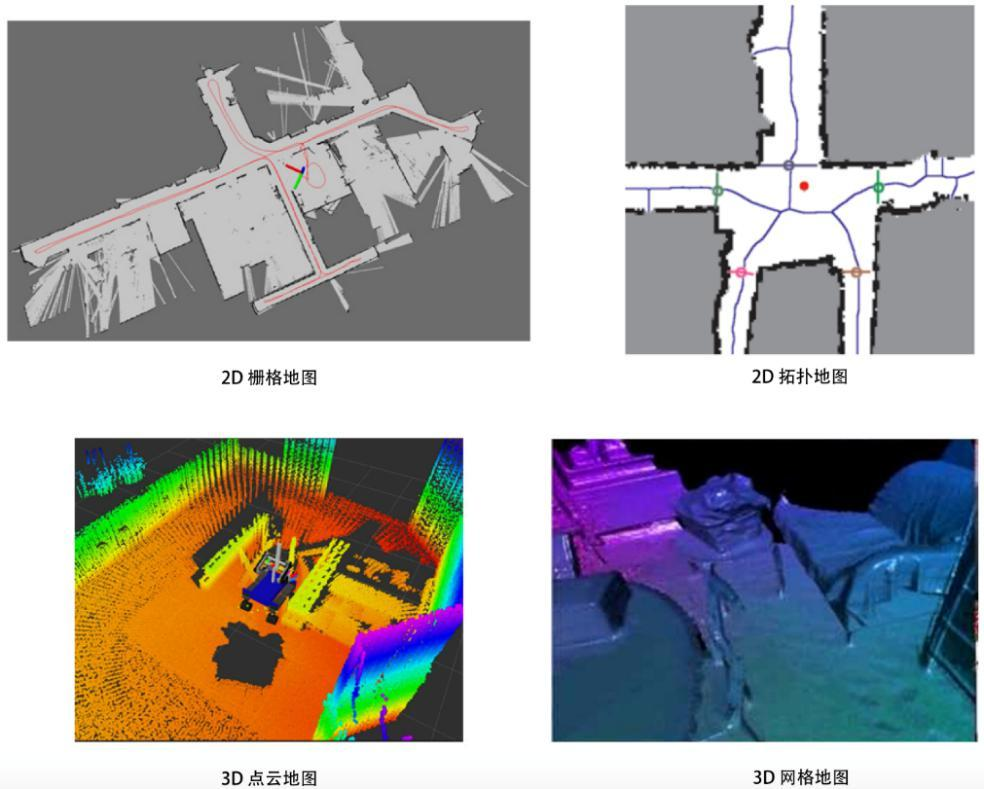
\includegraphics[height=10cm]{maps}
	\caption{回环检测示意图}
	\label{fig:maps}
\end{figure}\par

